\documentclass[11pt,a4paper,titlepage]{article}
\usepackage[utf8]{inputenc}
\usepackage[left=1.5cm,text={18cm, 25cm},top=2.5cm]{geometry}
\usepackage{setspace}
\usepackage{graphicx}
\usepackage[czech]{babel}
\setlength{\parindent}{0cm}
\setlength{\parskip}{1em}
\sloppy

\begin{document}

    \section{Rozbor a analýza algoritmu Bucket sort}
        Algoritmus Bucket sort řadí pomocí stromu procesů. Vstupem algoritmu je řada čísel.
        Nechť $n$ je počet čísel v této řadě, potom strom procesů obsahuje právě $m$ listových
        procesů, kde $m = \log_2 n$. Každý z těchto procesů řadí část vstupu pomocí některého
        ze sekvenčních řadících algoritmů. Počet prvků, které tyto procesy řadí je tedy roven $\frac{n}{m}$.
        Dále nechť $p$ reprezentuje celkový počet procesů, potom $p = (2 \times \log_2 n) - 1$.
        Procesy, které nejsou listovými procesy, spojují dvě seřazené seřazené sekvence pomocí
        sekvenčního algoritmu.
        
        \subsection{Složitost a cena algoritmu}
        Listové procesy čtou $\frac{n}{\log_2 n}$ prvků. Jedná se tedy o složitost $\mathcal{O}(\frac{n}{\log_2 n})$.
        Při použití sekvenčního řadícího algoritmu se složitostí $\mathcal{O}(r \times \log_2 r )$ bude výsledná složitost
        řazení $\mathcal{O}(\frac{n}{\log_2 n} \times \log_2 \frac{n}{\log_2 n}) = \mathcal{O}(n)$. Dále se zde nachází
        nelistové procesy, které je třeba do celkové složitosti algoritmu započítat. Proces při $j$--té iteraci se nachází
        v úrovni stromu $i = (\log_2 m) - j$ a spojí 2 posloupnosti o délce $\frac{n}{2^i}$. Při použití sekvenčního řadícího
        algoritmu určeného ke sloučení 2 seřazených posloupností se složitostí $\mathcal{O}(k)$ bude výsledná časová složitost
        práce nelistových procesů:
        $$\sum_{i=1}^{(\log_2 m) - 1} \frac{k \times n}{2^i} = \mathcal{O}(n)$$
        Poslední řazení kořenovým procesem s uložením dat do paměti má složitost $\mathcal{O}(n)$.
        
        Celková časová složitost algoritmu je tedy $\mathcal{O}(n)$. Počet potřebných procesů k dosažení této
        časové složitosti je $\mathcal{O}(log_2 n)$. Výsledná cena algoritmu Bucket sort potom bude $\mathcal{O}(log_2 n)$.
        Vzhledem k časové složitosti sekvenční implementace algoritmu Bucket sort se jedná o optimální cenu.

	\section{Implementace}
        Aplikace bks řadí data ze souborů. Tyto soubory považuje za binární a každý byte z jedno číslo ze vtupní sekvence.
        Rozsah čísel se kterými tedy aplikace pracuje je 0 -- 255. Načtená data následně seřadí pomocí algoritmu Bucket sort,
        kde je v listových procesech použit sekvenční řadící algoritmus shell sort a v nelistových procesech je použit
        merge sort pro sjednocení 2 seřazených posloupností.
        
        Samotná aplikace bks vyžaduje 1 argument reprezentující vsutpni soubor a lze ji spustit například pomocí následujícího příkazu:
\begin{verbatim}
mpirun --prefix /usr/local/share/OpenMPI -np PROCESS_COUNT bks INPUT_FILE
\end{verbatim}
        Při spuštění aplikace je nutné zadat správný počet procesů, jinak aplikace končí s návratovou hodnotou 2.
        Počet procesů je určen nejbližší větší druhou mocninou čísla $\left \lceil{log_2 n}\right \rceil$.
        Důvodem této úpravy algoritmu je fakt, že $log_2 n$ je celé číslo, pokud je hodnota $n$ druhou
        mocninou čísla $2$. Ve chvíli, kdy $log_2 n$ nevychází jako celé číslo je i uměle navýšena velikost vstupního
        souboru o čísla $255$ (maximální velikost jedné vstupní hodnoty) tak, aby všechny listové procesy pracovaly se stejnou
        velikostí dat. Kořenový proces, který provádí poslední řazení, poté takto přidaná čísla ignoruje.

	\section{Experimenty}

	\section{Komunikace}
    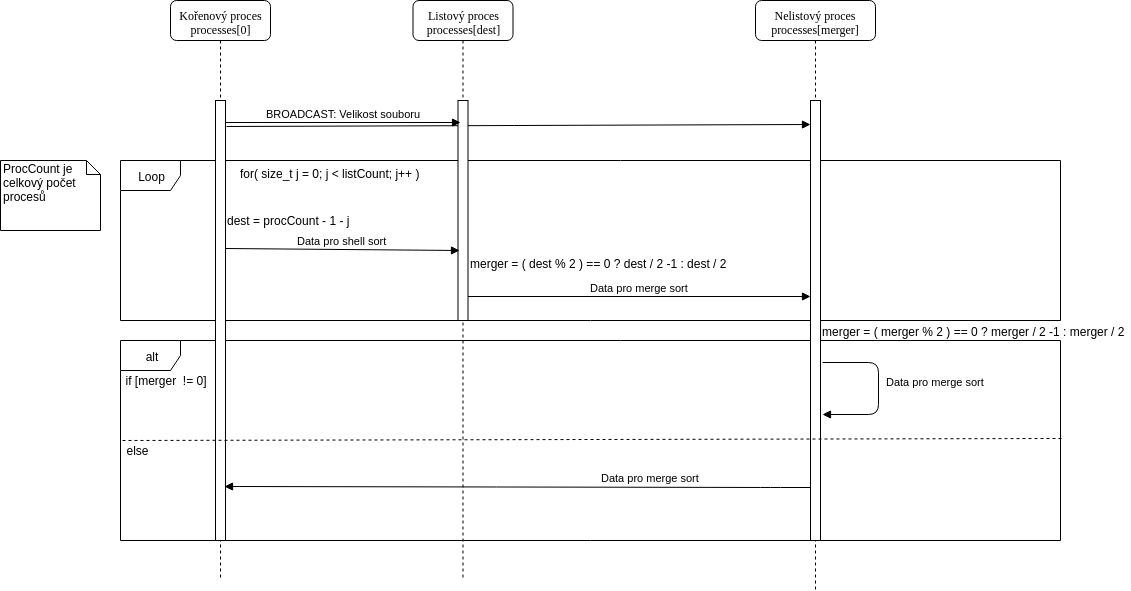
\includegraphics[width=\textwidth]{sequenceDiagram.png}
	\section{Závěr}

\end{document}
